\documentclass[tikz,border=3pt]{standalone}
\usepackage{xcolor}
\usetikzlibrary{arrows.meta,decorations.pathmorphing}
\definecolor{curveblue}{HTML}{2563EB}
\definecolor{axisgray}{HTML}{475569}
\begin{document}
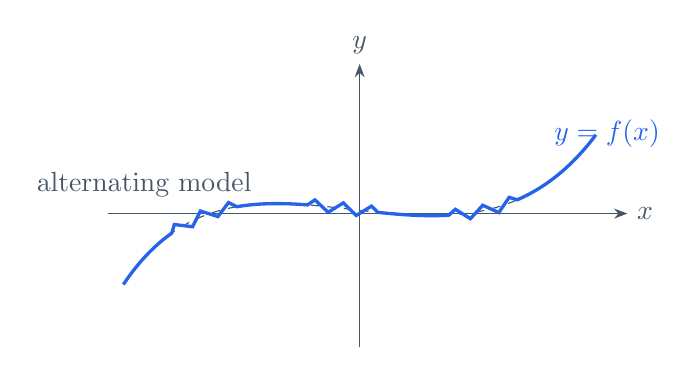
\begin{tikzpicture}[>=Stealth]
  \draw[axisgray,-Stealth] (-3.2,0) -- (3.4,0) node[right] {$x$};
  \draw[axisgray,-Stealth] (0,-1.7) -- (0,1.9) node[above] {$y$};
  \draw[axisgray,dashed] (-3,-.9) .. controls (-1.4,1.5) and (1.2,-1.4) .. (3,1);
  \draw[curveblue,very thick,decorate,
    decoration={straight zigzag,meta-segment length=9mm,segment length=3.6mm,amplitude=.7mm}]
    (-3,-.9) .. controls (-1.4,1.5) and (1.2,-1.4) .. (3,1);
  \node[curveblue,above right] at (2.35,.72) {$y=f(x)$};
  \node[axisgray,below left] at (-1.25,.65) {alternating model};
\end{tikzpicture}
\end{document}
